\documentclass[fleqn]{beamer}

\usepackage{amsmath}
\usepackage{animate}
\usepackage{amsfonts}
\usepackage[mathscr]{eucal}
\usepackage{subcaption}
\usepackage{wrapfig}
\usepackage{graphicx}

\usepackage{fancyhdr}
\usepackage{pstricks}
\usepackage{pst-func}
\usepackage{pst-plot}
\usepackage[utf8x]{inputenc}
\usepackage[spanish]{babel}


\setbeamertemplate{navigation symbols}{}
\definecolor{UniBlue}{RGB}{83,121,170}
\setbeamercolor{frametitle}{fg=black,bg=white}
\setbeamercolor{title}{fg=black,bg=yellow!85!orange}
%\setbeamercolor{title}{fg=red,bg=yellow!90!blue}
\usetheme{Madrid}

\beamersetuncovermixins{\opaqueness<1>{25}}{\opaqueness<2->{15}}
\begin{document}

\title{Clipping (recorte)}
\author{Reynaldo Martell}
\date{\today} 

\begin{frame}
\titlepage
\end{frame}

\begin{frame}\frametitle{\rule{0mm}{10mm}\rule{5mm}{0mm} Motivación. }
\begin{itemize}
\item Determinación de visibilidad.
\item Costo computacional elevado.
\item Extraer partes de una imagen (descartar geometría).
\end{itemize}
\end{frame}

\begin{frame}\frametitle{\rule{0mm}{10mm}\rule{5mm}{0mm} Clipping (Recorte). }
\begin{itemize}
\item Recorte en 2 dimensiones: una ventana.
\item Recorte en 3 dimensiones: recorte de volumen.
\item Para líneas y polígonos se simplifica.
\item Difícil para el caso de letras y curvas.
Difícil para el caso de letras y curvas.
\end{itemize}
\end{frame}

\begin{frame}\frametitle{\rule{0mm}{10mm}\rule{5mm}{0mm} Clipping (Recorte). }
\begin{figure}[H]
	\centering
	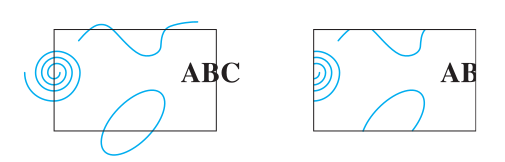
\includegraphics[width=0.95\textwidth]{images/recorteCurvas.png}
	\label{mapa}
\end{figure}
\end{frame}

\begin{frame}\frametitle{\rule{0mm}{10mm}\rule{5mm}{0mm} Clipping (Recorte de puntos). }
\begin{itemize}
\item Las fronteras de un rectángulo de recorte se define con:\\
xmin, xmax, ymin y ymax.
\item Un punto con coordenadas $(x,y)$ está dentro de éste si:
$xmin <= x <=xmax$
\\
$ymin <= y <=ymax$
\end{itemize}
\end{frame}

\begin{frame}\frametitle{\rule{0mm}{10mm}\rule{5mm}{0mm} Clipping (Recorte de líneas). }
\begin{itemize}
\item AB se acepta trivialmente.
\item CD un punto extremo dentro y el otro fuera.
\item EF, GH y  IJ sus puntos extremos caen fuera del área de recorte.
\begin{figure}[H]
	\centering
	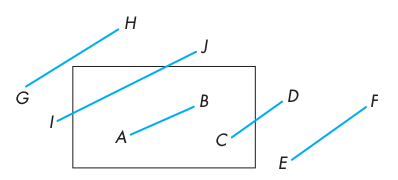
\includegraphics[width=0.7\textwidth]{images/descarteLineas.png}
	\label{mapa}
\end{figure}
\end{itemize}
\end{frame}

\begin{frame}\frametitle{\rule{0mm}{10mm}\rule{5mm}{0mm} Clipping (Métodos Recorte de líneas). }
\begin{itemize}
\item Analítico (Resolución de ecuaciones simultáneas).
\item Cohen-Sutherland.
\item Liang-Barsky.
\end{itemize}
\end{frame}

\begin{frame}\frametitle{\rule{0mm}{10mm}\rule{5mm}{0mm} Clipping (Método por fuerza bruta). }
\begin{itemize}
\item Intersectar la línea con cada uno de los cuatro planos que definen el área de recorte.\\
(xmin, xmax,ymin,ymax)
\item Chequear los puntos de intersección y verificar si caen dentro o fuera del área de recorte.
\\
$p=P_{0} + t(p_{1} - p_{0})$
\item Si t está dentro del rango [0, 1] existe intersección.
\item Este metodo es ineficiente.
\end{itemize}
\end{frame}

\begin{frame}\frametitle{\rule{0mm}{10mm}\rule{5mm}{0mm} Clipping (Método Cohen-Sutherland). }
\begin{itemize}
\item Evaluación de los puntos extremos.
\item Si la línea no es rechazada o aceptada trivialmente, se subdivide.
\item Trivialmente aceptada. Ambos puntos extremos caen dentro del área de recorte.
\item Trivialmente rechazada. Ambos puntos extremos caen fuera del plano medio de la frontera del área de recorte.
\end{itemize}
\end{frame}

\begin{frame}\frametitle{\rule{0mm}{10mm}\rule{5mm}{0mm} Clipping (Método Cohen-Sutherland). }
\begin{itemize}
\item Caso 1: Ambos puntos extremos caen dentro del área de recorte.\\
Caso trivial de aceptación.
\item Caso 2: Ambos extremos caen fuera de la línea y en un mismo lado de las líneas del área de recorte.\\
Caso trivial de rechazo.
\begin{figure}[H]
	\centering
	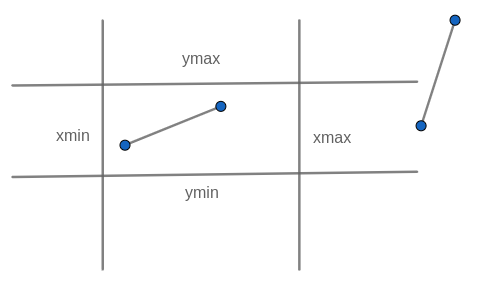
\includegraphics[width=0.7\textwidth]{images/casosDescartar.png}
	\label{mapa}
\end{figure}
\end{itemize}
\end{frame}

\begin{frame}\frametitle{\rule{0mm}{10mm}\rule{5mm}{0mm} Clipping (Método Cohen-Sutherland). }
\begin{itemize}
\item Caso 3: Uno de los puntos del segmento cae dentro y otro fuera del área de recorte.\\
Debe haber por lo menos una intersección.
\item Caso 4: Ambos puntos extremos caen fuera del área de recorte.\\
Puede está dentro o fuera.
\begin{figure}[H]
	\centering
	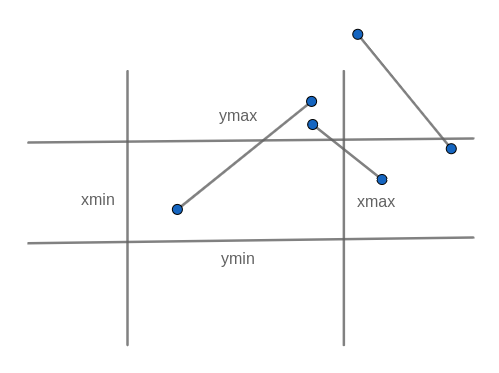
\includegraphics[width=0.7\textwidth]{images/casosDescartar2.png}
	\label{mapa}
\end{figure}
\end{itemize}
\end{frame}

\begin{frame}\frametitle{\rule{0mm}{10mm}\rule{5mm}{0mm} Clipping (Método Cohen-Sutherland). }
\begin{figure}[H]
	\centering
	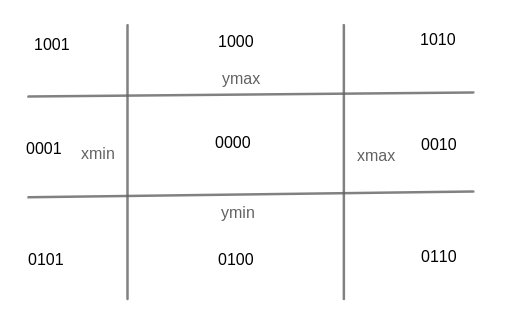
\includegraphics[width=0.6\textwidth]{images/TBRL1.png}
	\label{mapa}
\end{figure}
\centering
TBRL
\\
\begin{itemize}
\item $T = y > ymax$
\item $B = y < ymin$
\item $R = x > xmax$
\item $L = x < xmin$
\end{itemize}
\end{frame}

\begin{frame}\frametitle{\rule{0mm}{10mm}\rule{5mm}{0mm} Clipping (Método Cohen-Sutherland). }
\begin{figure}[H]
	\centering
	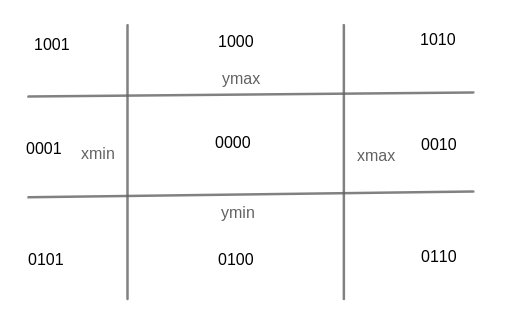
\includegraphics[width=0.49\textwidth]{images/TBRL1.png}
	\label{mapa}
\end{figure}
\begin{itemize}
\item Si ambos puntos del segmento tiene código 0, la línea está totalmente contenida en el área de recorte.
\item Si ambos extremos están del mismo lado del rectángulo de recorte, tendrán códigos igual 1 en la misma posición, por lo que aplicar la operación lógica and el resultado es diferente de cero. En este caso es trivialmente descartado.
\item El otro caso se debe calcular intersección.
\end{itemize}
\end{frame}

\begin{frame}\frametitle{\rule{0mm}{10mm}\rule{5mm}{0mm} Clipping (Método Cohen-Sutherland). }
\begin{figure}[H]
	\centering
	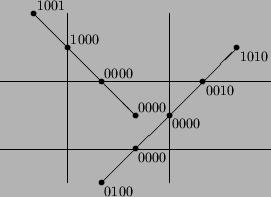
\includegraphics[width=0.7\textwidth]{images/TBRL2.png}
	\label{mapa}
\end{figure}
\end{frame}

\begin{frame}\frametitle{\rule{0mm}{10mm}\rule{5mm}{0mm} Clipping (Método Cohen-Sutherland). }
\begin{figure}
\centering
\begin{subfigure}{.5\textwidth}
  \raggedleft
  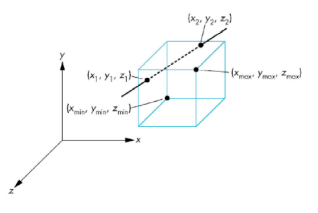
\includegraphics[width=.7\linewidth]{images/TBRL3D1.png}
\end{subfigure}%
\begin{subfigure}{.5\textwidth}
  \raggedright
  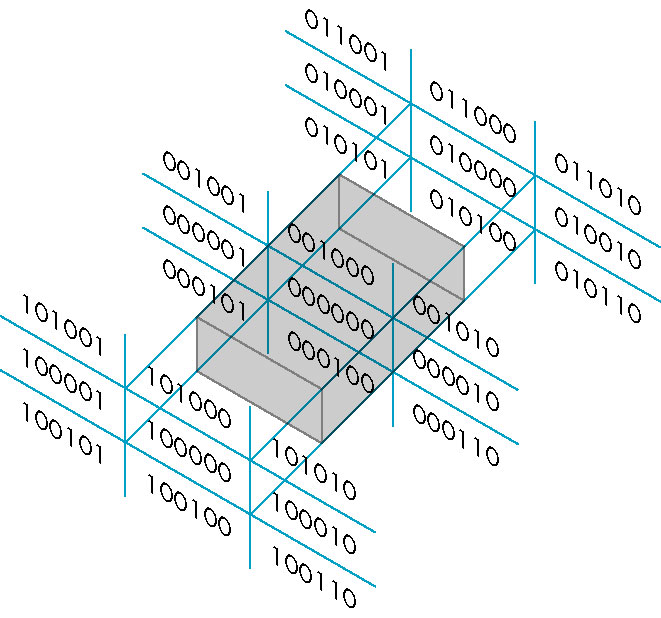
\includegraphics[width=.8\linewidth]{images/TBRL3D2.png}
\end{subfigure}
\end{figure}
\end{frame}

\begin{frame}\frametitle{\rule{0mm}{10mm}\rule{5mm}{0mm} Clipping (Método Cohen-Sutherland). }
\begin{itemize}
\item \textbf{Ejercicio 1}: Triángulo definido por los puntos A = (0, 0), B = (6, 0) y C = (6, 6) y ventana (3, 1), (9, 1), (9, 5) y (3, 5)
\item \textbf{TAREA EJ1}: Recorte ejercicio de proyecciones..
\item \textbf{TAREA EJ2}: Triángulo definido por los puntos A = (7, 0), B = (10, 3) y C = (7, 6) y ventana (3, 1), (9, 1), (9, 5) y (3, 5)
\end{itemize}
\end{frame}


\end{document}